% Created 2015-10-12 Mon 15:50
\documentclass{article}
\usepackage[top=1in, bottom=1.in, left=1in, right=1in]{geometry}
  \usepackage[makeroom]{cancel}
\usepackage{verbatim}


\usepackage[utf8]{inputenc}
\usepackage{lmodern}
\usepackage[T1]{fontenc}
\usepackage{fixltx2e}
\usepackage{graphicx}
\usepackage{longtable}
\usepackage{float}
\usepackage{wrapfig}
\usepackage{rotating}
\usepackage[normalem]{ulem}
\usepackage{amsmath}
\usepackage{textcomp}
\usepackage{marvosym}
\usepackage{wasysym}
\usepackage{amssymb}
\usepackage{amsmath}
\usepackage[version=3]{mhchem}
\usepackage[numbers,super,sort&compress]{natbib}
\usepackage{natmove}
\usepackage{url}
\usepackage{minted}
\usepackage{underscore}
\usepackage[linktocpage,pdfstartview=FitH,colorlinks,
linkcolor=blue,anchorcolor=blue,
citecolor=blue,filecolor=blue,menucolor=blue,urlcolor=blue]{hyperref}
\usepackage{attachfile}
\author{Abhishek Bagusetty}
\date{\today}
\title{24-623 2015 HM3}
\begin{document}

\maketitle

\section{Problem 2}
\label{sec-1}
Velocities, positions and forces are the important variables allocated dynamically using double pointers. The size of the system or the number of atoms are determined dynamically. Initial velocity is randomly assigned uand scaled between -1.0 and 1.0. After the initial velocites are set certain constraints are imposed. (1). Velocities are scaled in such a way that the total momentum of the system is zero. This performed with the Eq.\ref{eq:1}:

\begin{equation}
v_{i} = v_{i} - \frac{1}{N}\sum_{j=1}^{N}v_{j} \label{eq:1}
\end{equation}
where N is the total number of atoms.
(2). After the velocities are scaled for momentum, they are re-scaled such that the steady-state temperature of 100K is obtained for 200 units of NVE ensemble MD simulation.

Pair Energies, kinetic energy, momentum, temperature and pressure of the system are flushed to for post-processing for every 500 time steps. Center of mass(COM) is computed at each time frame to prove that there is no drift and also can also be visualized from the snapshots given below.
Periodic cell is also shown in the Fig.\ref{fig:2d} , Fig.\ref{fig:2e} for the inital and final state of teh system.

Components of momentum in x,y,z directions are computed and shown in Fig.\ref{fig:2b}. 


\begin{figure}[htb]
\centering
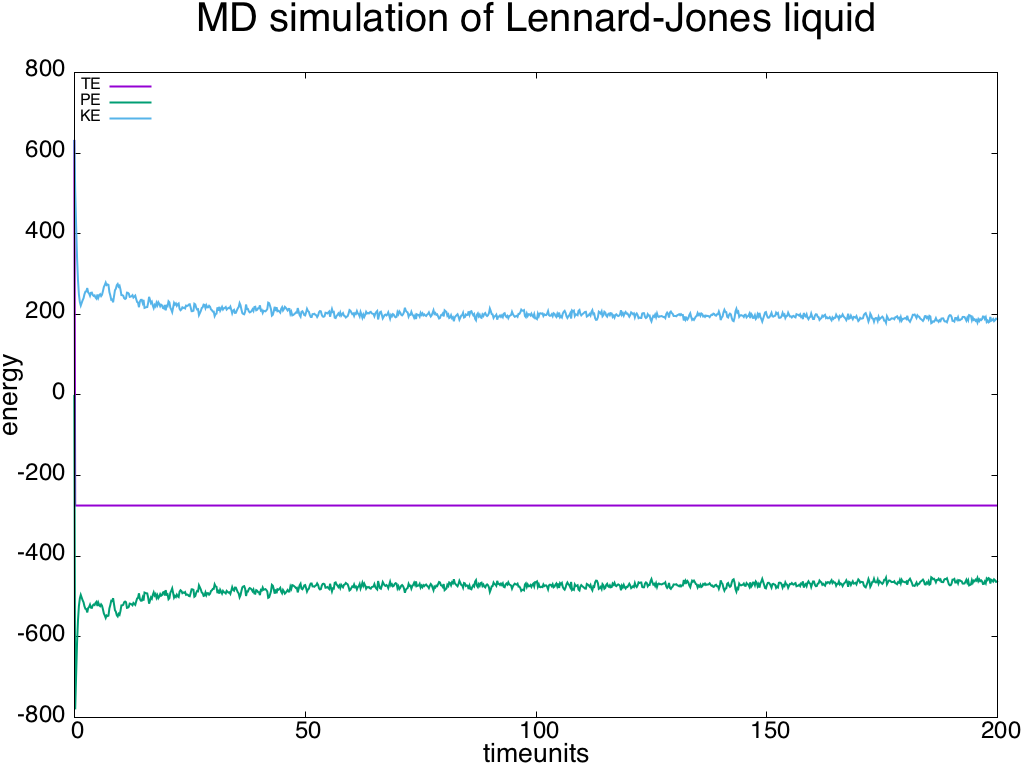
\includegraphics[width=.9\linewidth]{./P2/LDmj_sim_ener.png}
\caption{\label{fig:2a}The figure shows the plot of energy for the NVE ensemble MD simulation of LJ nano-particles over 200 units.}
\end{figure}

\begin{figure}[htb]
\centering
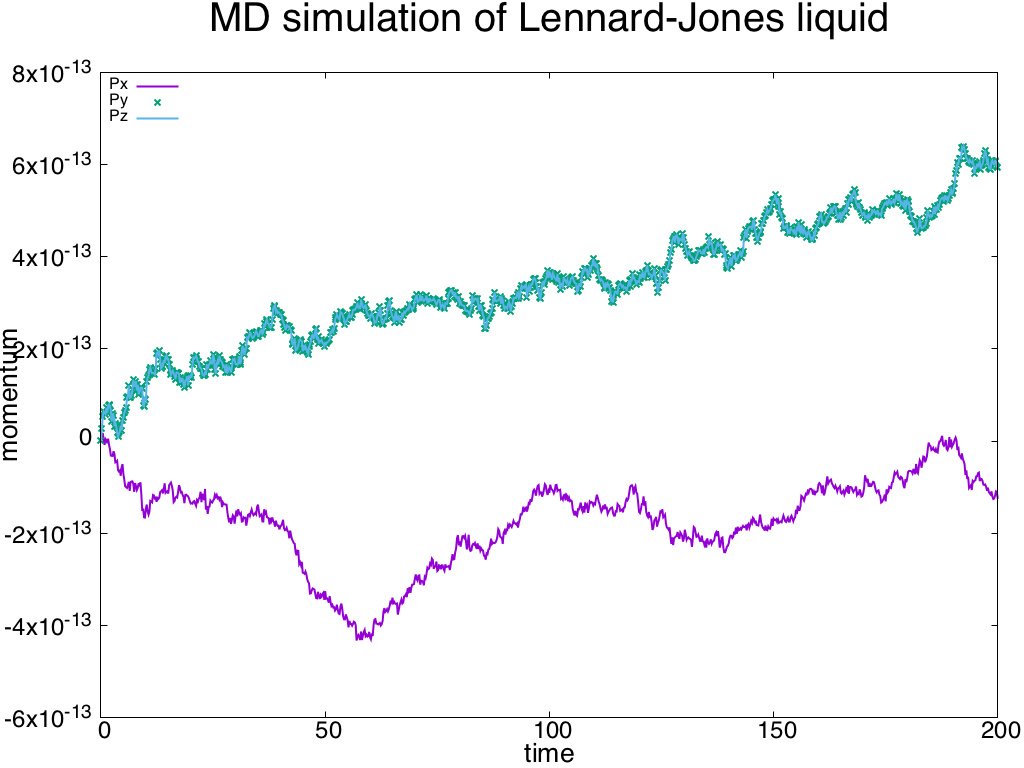
\includegraphics[width=.9\linewidth]{./P2/LDmj_sim_mom.png}
\caption{\label{fig:2b}The figure shows the plot of components of momentum for the NVE ensemble MD simulation.}
\end{figure}

\begin{figure}[htb]
\centering
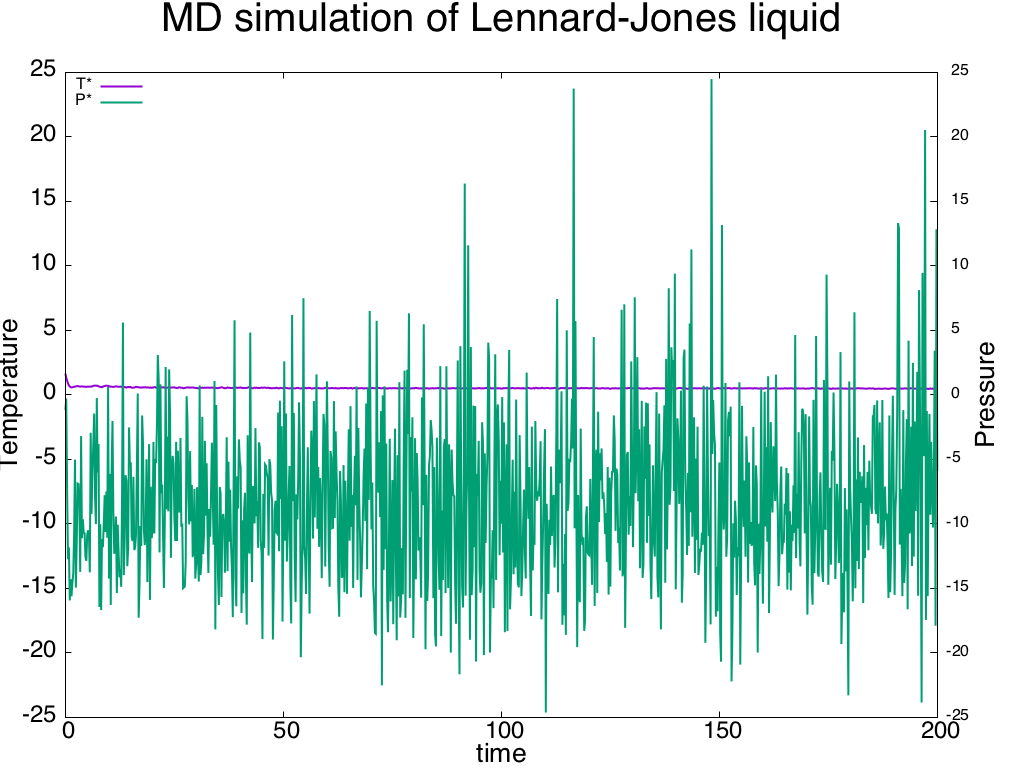
\includegraphics[width=.9\linewidth]{./P2/LDmj_sim_temp_P.png}
\caption{\label{fig:2c}The figure shows the plot of instantaneous temperature and pressure in reduced units for NVE ensemble MD simulation.}
\end{figure}


\begin{figure}[H]
\begin{centering}
\scalebox{0.35}{\includegraphics{P2/unit0.png}}
\caption{Snapshot taken at t=0 (units). Simulation boundaries are also shown in blue. The center of mass of the system is shown as an atom colored in red.}
\label{fig:fig2d}
\end{centering}
\end{figure}

\begin{figure}[H]
\begin{centering}
\scalebox{0.35}{\includegraphics{P2/unit200.png}}
\caption{Snapshot taken at t=200 (units). Simulation boundaries are also shown in blue. Please note that the coordinates are wrapped into the simulation cell using PBC module available in VMD for visualization purpose. The center of mass of the system is shown as an atom colored in red.}
\label{fig:fig2e}
\end{centering}
\end{figure}
% Emacs 24.4.1 (Org mode 8.2.10)
\end{document}